\section{Results}
\label{sec:results}
\begin{table}[t]
\centering
\caption{Distribution of Regular Expressions' attributes}
\label{regex:distr}
\begin{tabular}{lllllllll}
Attribute       & mean & min & max     & 25\% & 50\% & 75\% & 90\% & 99\%  \\
Nodes(DFA Size) & 156  & 2   & 433508  & 9    & 21   & 72   & 387  & 948   \\
Edges           & 604  & 1   & 2348520 & 15   & 56   & 214  & 1013 & 2811  \\
Edge Pairs      & 2221 & 0   & 8693181 & 14   & 94   & 409  & 1597 & 16359 \\
Total Inputs    & 386  & 1   & 595642  & 2    & 4    & 24   & 168  & 3128  \\
Unique Inputs   & 5    & 1   & 34      & 1    & 2    & 5    & 13   & 32    \\
Projects		& 1	   & 1	 & 129    & 1    & 1     & 1    & 1    & 5
\end{tabular}
\end{table}
This section presents our results of the three research questions in order. 

We generated static and dynamic DFAs for in total 15091 regular expressions from 1665 Java GitHub projects\footnote{add url for repo data}. Among all the regular expressions, XXX could not build their static DFAs either because it contains regular expression features unsupported by RE2 or because the length of regular expression string is larger than the string length limit of bash scripts(i.e.131071) or because the regular expression string contains null byte which is not valid in bash scripts. For the remaining 14638 regular expressions, we dropped 9 because they are used across over 166 projects (10\% of total projects), and dropped 1419 because their unique inputs for matching is beyond the 90 percentile of all regular expressions. The coverage analysis are based on the final 13210 regular expressions and 1428 projects. 

Table~\ref{regex:distr} describes the distribution of the regular expressions' attributes. 75\% of the all regular expressions keep a simple DFA graph. The matching between a regular expression and a input string could be repeated multiple times in the same project or across multiple projects. Almost all the regular expressions are used in only one project. The regular expressions used in the third-party libraries still exist but there are only few of them.

\section{Bug Report Study (RQ1)}
\label{sec:rq1}
In this section, we present four common types of regular expression.related bugs. We describe the bug causes and its impacts of each bug type. At the end of discussing each type, we propose some possible solutions to them.

\subsection{Artifacts}
 To explore the impact of buggy regular expressions, we explored bug databases for large bug reporting systems, specifically Bugzilla, GitHub, and Apache JIRA.
  We filtered bugs related to regular expressions with searching keywords "regular expression", "regex", and "regexp". 
  There are \todo{num} bugs collected, and we randomly selected \todo{num} to analyze. The goal was to determine the extent to which low coverage poses a problem for regular expressions. 
  
  \subsection{Analysis}
  For each bug report, we \todo{describe your process}

\subsection{Results}
\subsubsection{Catastrophic Backtracking}
Backtracking is the most difficult type of regular expression.related bugs. Backtracking happens in the regular expression engines of Nondeterministic Finite Automaton (NFA) implementation. When NFA decides the states it should take, it tries one state a time. If the rest matching process arrives an error state, it backtracks to where it choose the state and selects another state to try.

\noindent {\textbf{Impact: }} Backtracking usually takes exponential time to complete. It also consumes a lot of computing resources (e.g., CPU and Memory) and therefore slows down the program responses~\cite{stackoverflow}. Sometimes, backtracking in regular expression could even cause crashes of systems and softwares (e.g., browsers, websites, etc)~\cite{browser}. It can be exploit for ReDos attacks as well.

\noindent {\textbf{Solutions: }} a) Use a regular expression engine implemented in DFA. While the NFA implementation takes regular expression engines exponential time to finish, the DFA version takes linear time. However, it is not always feasible to choose regular expression engines. b) Avoid the regular expression features which causes backtracking. Backtracking is only used for some of the regular expression engines. Finding equivalent regular expression without these features could avoid the backtracking.

\subsubsection{Strings of zero length and long string} If a valid regular expression is given to match a zero-length string, some regular expression engines will try to read a character infinitely. This problem is manifested in Bug 374923\todo{add}. If the regular expression is given a very long string, its execution time is linear to the string length in DFA implemented regular expression engine. This situation is common in regular expression containing wildcard * and +. Take the regular expression "a+b" as an example. The matching for string "ab" 
\noindent {\textbf{Impact: }} Similar to backtracking, strings of zero length could cause system hangs.
\noindent {\textbf{Solutions: }}
\subsubsection{Escape Characters}
\noindent {\textbf{Impact: }}
\noindent {\textbf{Solutions: }}
For the characters which have dual meaning in the regular expression.
\subsubsection{Case sensitivity}
\noindent {\textbf{Impact: }}
\noindent {\textbf{Solutions: }}
Need test cases to test its sensitivity to match its regular expression purpose.
\subsubsection{Special Characters}
\noindent {\textbf{Impact: }}
\noindent {\textbf{Solutions: }}
Some regular expression may accept unexpected characters because the composition of regular expression does not consider it. Some paths are not explored during testing. low coverage.
Some regular expression reject characters but they should accept them.

The sample should consider as many samples as possible. Although the regular expression may have a 100% coverage, we should also analyze the rejected strings. The weakness of strings generated by regular expression tools is that these strings are usually constructed to match the regular expression, not to mismatch it.

Another solution is collecting similar regular expressions of the same purpose.
\subsubsection{Match pattern and alternation order}
\noindent {\textbf{Impact: }}
\noindent {\textbf{Solutions: }}
Match pattern matters. \todo{add an example about first match and longest match}
alternation order matters. h|s|m|ms or h|s|ms|m----------what is the results of First match longest match for them.

\section{Results}
\label{sec:results}

Here, we present the results of RQ1 and RQ2 in turn.

%\begin{figure}[t]
%  \begin{subfigure}[t]{0.45\textwidth}
%  	\centering
%    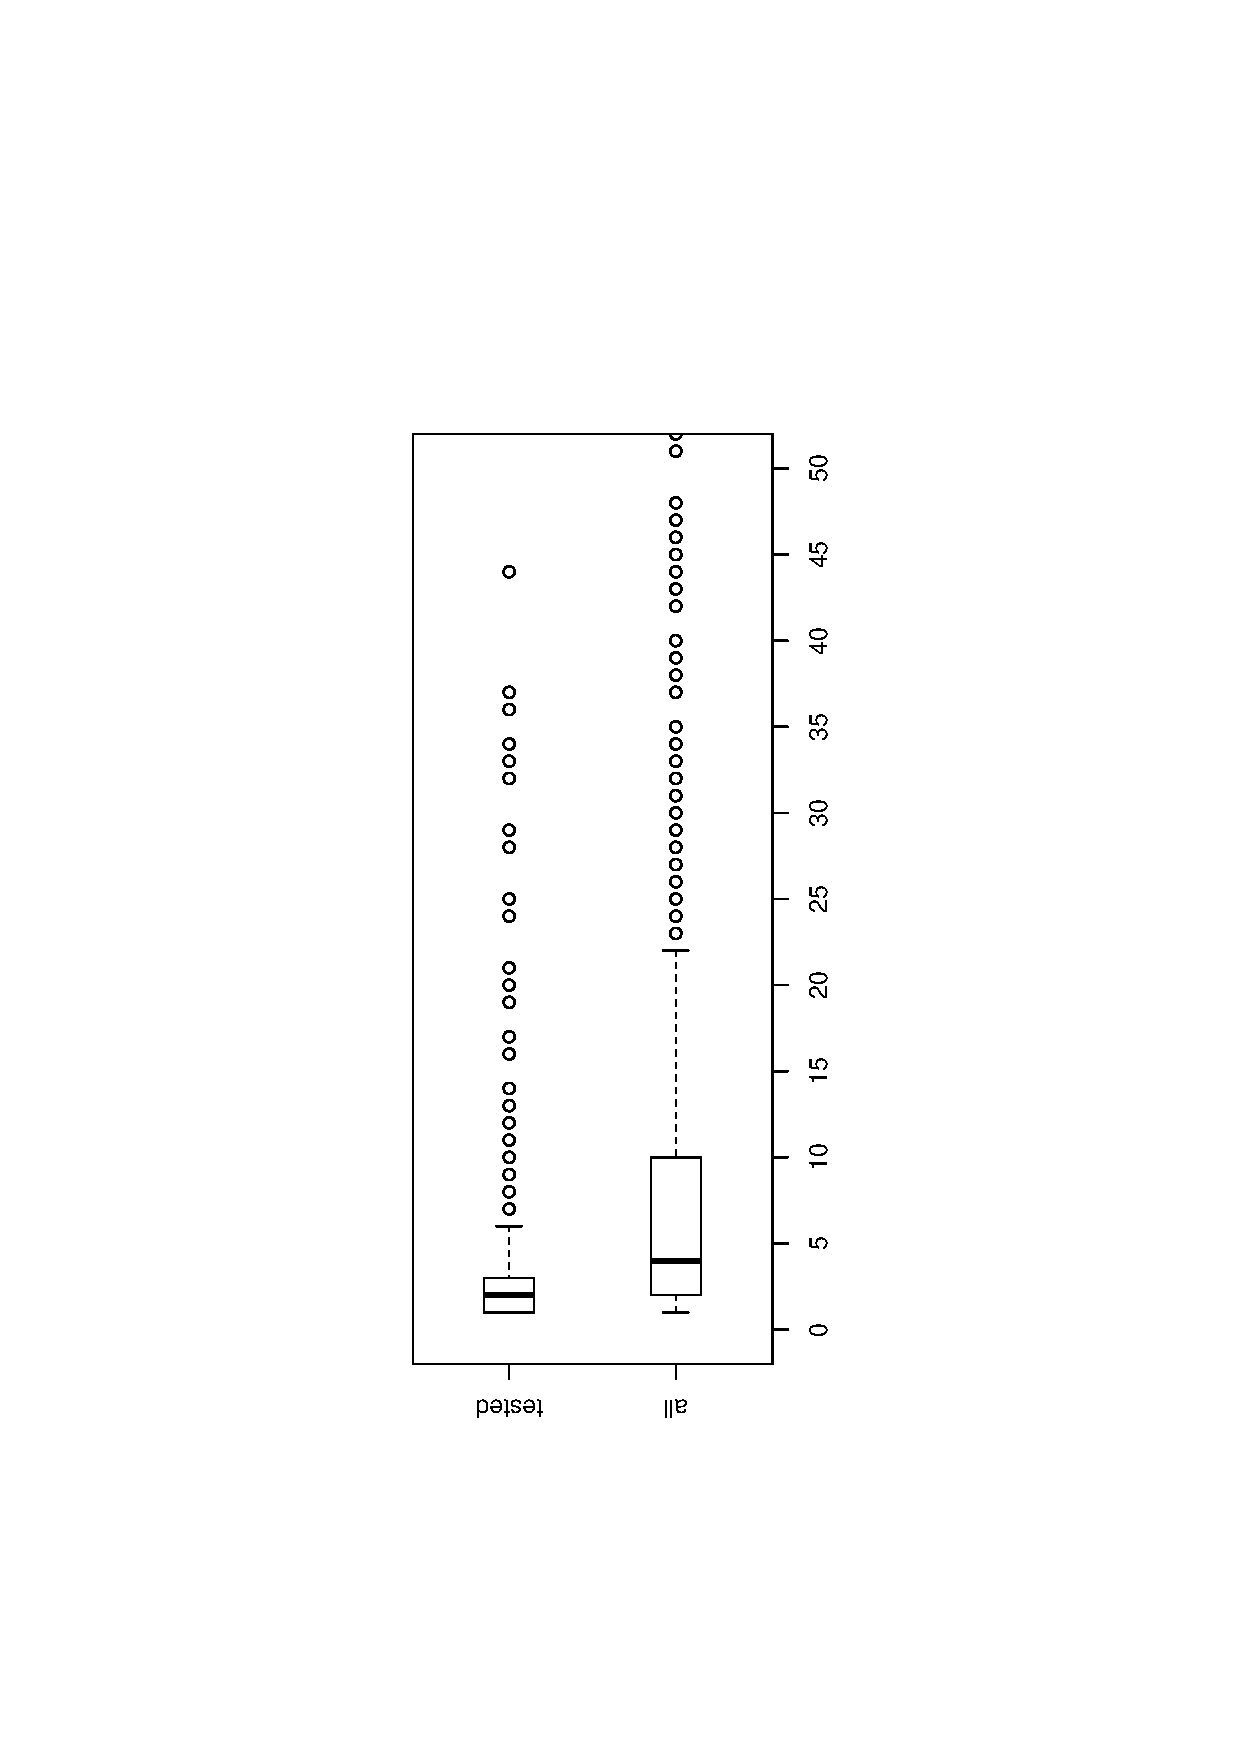
\includegraphics[width=\textwidth]{figures/callsite1}
%    \vspace{-20pt}
%    \caption{Number of FullMatch call sites per GitHub project}
%    \label{fig:callsite1}
%  \end{subfigure}
%  \vspace{6pt}
%  \begin{subfigure}[t]{0.45\textwidth}
%  	\centering
%    \includegraphics[width=\textwidth]{figures/callsite2}
%    \vspace{-20pt}
%    \caption{Number of regular expressions per tested call site}
%    \label{fig:callsite2}
%  \end{subfigure}
%\vspace{-12pt}
%\caption{{\em all} represents all 18,426 call sites in 1,225 projects, and {\em tested} represents the 3,093 tested call sites in 1,225 projects. There are 15,096 tested regular expressions.}
%\vspace{-12pt}
%\label{fig:callsite}
%\end{figure}

\subsection{RQ1: Test Coverage of Regular Expressions}
\label{sec:rq2}
\label{rq1:results}
%Since there are 18,514 regular expressions in 1,256 GitHub projects which are used for Full Match and of them 15,562 are tested, 2952 regular expressions in 1,256 GitHub projects are not tested. We reported 15,096 of 15,562 tested regular expressions, therefore, the number of reported regular expressions which are not tested is about $2952*\frac{15,096}{15,562} \approx 2863$. Regarding the coverages of those 2,863 untested regular expressions as zeros, we report the coverage metrics of total 17,959 regular expressions.


We address RQ1 is two ways. First, we look at the number of call sites to FullMatch methods are actually tested. Next, we look at the test coverage for each tested regular expression, 

\subsubsection{Tested Call Sites}
In the 1,225 projects, there are  18,426 call sites of the instrumented functions in Section~\ref{sec:instrumentedfunctions}. However, only 3,093 call sites are executed by the test suites. 
This means that 15,333 (83.21\%) of the call sites are not covered by the test suites. For those that are, the median of unique regular expressions per tested call site is one, with an average of five (Table~\ref{regex:distriprojects}). 

%Figure~\ref{fig:callsite} describes the projects in terms of \emph{call sites}, \emph{tested call sites}, and \emph{regular exp./tested call site} (number of regular expressions per tested call site). Figure~\ref{fig:callsite1} illustrates the distribution of call sites over 1,225 GitHub projects. Figure~\ref{fig:callsite2} illustrates the distribution of unique regular expressions executed at each call site. 
%This is a very skewed distribution as many of the call sites are never invoked by the tests; it is for this reason that we focus our discussion on just the regular expressions that are executed by the test suites. 

%\paragraph{Summary:}
\textbf{Summary:}
Of the 18,426 call sites for FullMatch methods in 1,225 GitHub projects, only 3,093 (16.8\%) are executed by the test suites. 
%Most call sites are executed by only one regular expression, but one call site is tested by 1,523 regular expressions. 
%The 15,096 regular expressions we study come from only 3,093 call sites in the 1,225 projects. In all 1,225 projects, there are . 



%\begin{figure}[t]
%	\centering
%	\includegraphics[width=0.45\textwidth]{figures/digits1001mapping2}
%	\vspace{-6pt}
%	\caption{Original DFA subgraph of the regular expression {\tt `\textbackslash d+'} given the input `1001'. $N_0$ is the initial node A. It is unknown yet whether the final node D is the error node $N_e$ or final accept node $N_m$.
%	%The numbers in square brackets are the bytes in decimal accepted in state transitions. For example, `[48-57]' indicates there is a transition if the input byte is one of `0', `1', `2', ..., `9'. 
%	`0,1' of the transition from state C to itself implies during the matching process there are two such transitions: one accepts the character `0' and the other accepts the character `1'. The byte 256 indicates there is no more bytes from the input string. The arrows colored blue represent transitions in successful matches.}
%	\label{fig:dynamic}    
%	\vspace{-6pt}
%\end{figure}





%\subsection{Results}

%We collected 15,091 regular expressions from 1,665 Java GitHub projects. 
%Among all the regular expressions, the static DFAs for 454 regular expressions could not be built because they contain regular expression features unsupported by RE2, the length of regular expression string is larger than the string length limit of bash scripts (i.e., 131,071), or the regular expression string contains null byte which is not valid in bash scripts. 
%For the remaining 14,637 regular expressions, we dropped 9 because they are used across over 166 projects (10\% of total projects) and thus assumed to be part of third-party libraries, and dropped 1,419 because their unique inputs for matching is beyond the 90 percentile of all regular expressions. \todo{I still don't understand this "unique inputs for matching" thing}.
\subsubsection{Coverage of Tested Regular Expressions}
We successfully generated static DFAs for 15,096 regular expressions from 1,225 Java GitHub projects  and dynamic DFAs for 899,804 regular expression/input string pairs.\footnote{We note that 899,804 is less than $60 \times 15096 = 905760$ because the mean of {\em\# Input strings ($\lvert S \rvert$)} is 59.60546 and rounded up to 60.}%\footnote{We note that 899,804 is less than $60 \times 15096 = 905760$. To save time, for non-unique regular expressions that were tested against the same strings in multiple projects, we  computed the dynamic DFA once and counted the coverage toward both.} 
Among the regular expressions, 4,941 (32.7\%)  regular expressions have only failing inputs (i.e., $\lvert S_{succ} \rvert = 0$) and 6,029 (39.9\%) have only inputs of successful matching (i.e.,  $\lvert S_{fail} \rvert = 0$). This means that 10,970 (72.7\%) of the regular expressions do not contain test inputs that exercise both the matching and non-matching scenarios. Of these, 6,318 (41.9\%) regular expressions contain only one test string (i.e., $\lvert S \rvert = 1$) There are  4,126 (27.3\%) regular expressions with both failed and successful matchings. %\footnote{Data are available at \texttt{blinded for review}} % \url{https://github.ncsu.edu/pwang7/ISSTA2018/tree/master/data}.}.

Table~\ref{regex:distri} describes properties of the test input sets for each regular expression: \emph{$\lvert S \rvert$} is the size of the test suite, computed as the number of unique input strings for a regular expression; $\lvert S_{succ} \rvert$ means the number of matching inputs; $\lvert S_{fail} \rvert$ means the number of failing inputs; \emph{succ_ratio} shows the ratio of successful matchings to all matchings for each regular expression; \emph{fail_ratio} shows the ratio of failed matchings to all matchings for each regular expression. 
%Since 6,318 (41.9\%) of the regular expressions have a single input string, we show the data for all regular expressions (top) and for just those where $\lvert S \rvert > 1$.
%Table~\ref{regex:distri} describes the distribution of the regular expressions' attributes after data cleaning.
%75\% of the all regular expressions keep a simple DFA graph. \todo{what is a "simple" DFA graph?} The matching between a regular expression and an input string could be repeated multiple times in the same project or across multiple projects. Almost all the regular expressions are used in only one project. The regular expressions used in the third-party libraries still exist but there are only few of them.

%\todo{Table~\ref{cov:data} description goes here}

\begin{table}[tb]
%\centering
%\caption{Description of 15,096/8,778 Regular Expressions' test suites.  All numbers are rounded to nearest integer except that success ratio rounded to two decimal places.}
\caption{Description of 15,096 Regular Expressions' test suites. All numbers are rounded to nearest integer except that success ratio rounded to two decimal places.}
\label{regex:distri}
\vspace{-6pt}
\begin{small}
%\resizebox{0.5\textwidth}{!}{%
%\begin{tabular}{lllllllll}
\begin{tabular}{p{2cm}
>{\raggedleft\arraybackslash}p{0.6cm}
>{\raggedleft\arraybackslash}p{0.6cm}
>{\raggedleft\arraybackslash}p{0.6cm}
>{\raggedleft\arraybackslash}p{0.6cm}
>{\raggedleft\arraybackslash}p{0.6cm}
>{\raggedleft\arraybackslash}p{0.6cm}}
\hline
Attributes & mean & 25\% & 50\% & 75\% & 90\% & 99\%  \\
\hline
$\lvert S \rvert$   & 60 & 1  & 2   & 7   & 27  & 662   \\
$\lvert S_{succ} \rvert$ & 19 & 0   & 1   & 1  & 4 & 79  \\
$\lvert S_{fail} \rvert$ & 41 & 0   & 1   & 4  & 19 & 383 \\
succ_ratio& 49.03 & 0.00 & 44.70 & 100.00 & 100.00 & 100.00 \\
fail_ratio& 50.97 & 0.00 & 55.30 & 100.00 & 100.00 & 100.00 \\
\hline
%\hline
%$\lvert S \rvert$   & 102 & 2  & 5   & 15   & 63  & 1232   \\
%$\lvert S_{succ} \rvert$ & 31 & 0   & 1   & 2    & 8   & 196  \\
%$\lvert S_{fail} \rvert$ & 70 & 2   & 3   & 11   & 44  & 753 \\
%succ_ratio& 27.29 & 0.00 & 5.88 & 50.00 & 100.00 & 100.00 \\
%fail_ratio& 72.71 & 50.00 & 94.12 & 100.00 & 100.00 & 100.00 \\
%\hline
\end{tabular}
%}

%\vspace{3pt}
%The first table shows the attributes of 15,096 regular expressions, the second table shows the attributes of 8,778 regular expressions which have more than more unique inputs.
\end{small}
%
%\vspace{5pt}
%
%\vspace{-12pt}
\end{table}


\begin{table}[tb]
%\centering
\caption{Coverage values in Figure~\ref{cov:stack}.}
\label{cov:data}
\vspace{-6pt}
\begin{small}
%\resizebox{0.5\textwidth}{!}{%
%\begin{tabular}{lllllllll}
\begin{tabular}{p{1cm}p{1cm}
>{\raggedleft\arraybackslash}p{0.6cm}
>{\raggedleft\arraybackslash}p{0.5cm}
>{\raggedleft\arraybackslash}p{0.6cm}
>{\raggedleft\arraybackslash}p{0.6cm}
>{\raggedleft\arraybackslash}p{0.7cm}
>{\raggedleft\arraybackslash}p{0.7cm}}
\hline
Coverage & Suite & mean & 25\% & 50\% & 75\% & 90\% & 99\%  \\
\hline
NC (\%)& $S$   & 59.05 & 24.62   & 63.64  & 95.65   & 100.00 & 100.00   \\
NC (\%)& $S_{succ}$ & 47.84 & 0.00    & 46.15  & 90.00   & 99.60  & 99.89   \\
NC (\%)& $S_{fail}$ & 18.89 & 0.00    & 8.51   & 25.00   & 62.26  & 100.00   \\
\hline
EC (\%)& $S$   & 28.74      & 6.67   & 23.90   & 49.97   & 53.80  & 80.00  \\  
EC (\%)& $S_{succ}$ & 23.20 & 0.00   & 12.36   & 49.96   & 50.00  & 60.00   \\
EC (\%)& $S_{fail}$  & 8.55 & 0.00   & 2.20    & 7.80    & 32.19  & 65.08   \\
\hline
EPC (\%)& $S$ &23.77    & 2.47    & 12.50  & 49.96  & 50.00 & 66.67 \\
EPC (\%)& $S_{succ}$ & 20.48 & 0.00    & 5.26   & 49.94  & 50.00  & 55.56   \\
EPC (\%)& $S_{fail}$  & 5.50  & 0.00    & 0.00   & 2.74   & 22.12  & 57.14   \\
\hline
%% distribution of 17,959
%\hline
%NC (\%)& $S$   & 49.64 & 10.81   & 43.48  & 90.91   & 99.88 & 100.00   \\
%NC (\%)& $S_{succ}$ & 40.21 & 0.00    & 29.03  & 85.71   & 99.08  & 99.89   \\
%NC (\%)& $S_{fail}$ & 15.88 & 0.00    & 0.23   & 21.43   & 53.57  & 100.00   \\
%\hline
%EC (\%)& $S$   & 24.16 & 3.61   & 12.50   & 49.95   & 51.55  & 76.31  \\  
%EC (\%)& $S_{succ}$ & 19.50 & 0.00   & 7.09   & 49.91   & 50.00  & 60.00 \\
%EC (\%)& $S_{fail}$  & 7.19  & 0.00   & 0.03    & 6.38    & 25.16   & 62.30 \\
%\hline
%EPC (\%)& $S$ &19.98    	& 0.34    & 5.24  & 49.89  & 50.00 & 66.67 \\
%EPC (\%)& $S_{succ}$ & 17.22 & 0.00   & 2.22  & 49.52  & 50.00 & 54.17   \\
%EPC (\%)& $S_{fail}$  & 4.62  & 0.00  & 0.00  & 2.25   & 16.18 & 54.12    \\
%\hline
\end{tabular}
%}
\end{small}
%
%\vspace{5pt}
%
\vspace{-12pt}
\end{table}
\iffalse
\begin{figure}[tb]
	\centering
	\includegraphics[width=0.5\textwidth]{figures/regexCov}
	\vspace{-6pt}
	\caption{Node, edge, and edge-pair Coverage for all regular expression matching across projects, successful matching, and failed matching.}
	\label{cov:regex}    
	\vspace{-6pt}
\end{figure}
\fi
\begin{figure}[tb]
	\centering
	\includegraphics[width=0.5\textwidth]{figures/stackCov}
	\vspace{-24pt}
	\caption{Coverage for 15,096 regular expressions.}% Total is computed over $S$, success is computed over $S_{succ}$, and failure is computed over $S_{fail}$. }
	%\caption{Coverage for 17,959 regular expressions. Total is computed over $S$, success is computed over $S_{succ}$, and failure is computed over $S_{fail}$. }
	\label{cov:stack}    
	\vspace{-6pt}
\end{figure}

%\begin{figure}[tb]
%	\centering
%	\includegraphics[width=0.5\textwidth]{figures/stackCovNot1}
%	\vspace{-6pt}
%	\caption{Node, edge, and edge-pair coverages for all regular expression matching across projects, successful matching, and failed matching whose inputs are more than one. \todo{what do we learn from this that the boxplot of all regexes doesn't already communicate? I'm thinking nothing and it should be dropped}}
%	\label{cov:stackNot1}    
%	\vspace{-6pt}
%\end{figure}



%We calculated both the coverages for each unique regular expression across all projects as shown in Figure~\ref{cov:stack}. Table~\ref{cov:data} shows the detailed coverage statistics in each combination of coverage types and matching types. 
%and both the coverages for each project across all regular expressions as shown in Figure~\ref{cov:repo}. ``success" consists of only successful regular expression matchings, ``failure" consists of only failed matchings, and ``total" consists of all regular expression matchings.

%\todo{I want a table with the results for easy comparison, similar to the one of the regular expression attributes. A boxplot is useful for visual, but I think the text below would be more clear in a table format. }
Table~\ref{cov:data} describes the distributions of Node Coverage (NC), Edge Coverage (EC), and Edge-Pair Coverage (EPC) over $S$, $S_{succ}$, and $S_{fail}$. Figure~\ref{cov:stack} displays this information graphically; {\em total} means the total number of input strings for each regular expression, namely the test suite $S$, {\em success} means  $S_{succ}$, and {\em failure} means $S_{fail}$. %\todo{explain the figure. Explain that {\em success} means $S_{succ}$ and so forth}
Most of the regular expressions are not tested thoroughly since the mean values of coverage are low, especially the edge and edge-pair coverage. 
%The coverage of successful matchings starts from 0\% because the ratio of successful matching is 0\% for the first quarter. 
Although the coverages on failed matchings are relatively small, they contribute to a high overall test coverage. Failed matching tests are a necessary part of testing regular expressions.% Compared to successful matchings, failed matchings have a lot of outliers.

%In Figure~\ref{cov:stackNot1} we present the results including regular expressions whose input strings are more than one because there is a high possibility that the regular expressions which have only one input string are just accidentally recorded while running Maven test. While the coverage metrics on total matchings and successful matchings are lower, the coverage metrics on failed matchings are higher than them in Figure~\ref{cov:stack}.

%\todo{Characterize a typical regular expression with multiple inputs here. State the regular expression, list some of the test strings, enumerate the sizes of $S$, $S_{succ}$ and $S_{fail}$. Describe NC, EC, and EPC.-----I think this is done in Table~\ref{coverageExample}}

%\paragraph{Summary:}
\textbf{Summary:}
%\todo{add a summary statement here}
A majority of regular expressions (10,970, 97.7\%) are tested with exclusively passing (6,029, 39.9\%) or exclusively failing (4,931, 32.7\%) test inputs. 
Edge and edge-pair coverage are both very low. 
Full node coverage is infeasible with only passing inputs as $N_e$ would never be covered; the presence of both types of inputs is important for thorough testing. 
%From the coverage analysis of 15,096 regular expressions, we can find that 1) It is more difficult to get high coverages of edges and edge-pairs than of nodes; 2) There is an upper bound for EC and EPC with only successful matching input strings; 3) regular expressions could achieve higher coverages if it is tested with both successful and failed matching input strings.


% 
%The regular expression testing coverages are correlated with their number of input strings as shown in Table~\ref{cov:input}. \texttt{Total} means the correlation between the coverages and total number of inputs. \texttt{Succ_ratio} shows the correlation between the coverages and the ratio of inputs on successful matchings over total inputs. \texttt{Fail\_ratio} shows the correlation between the coverages and the ratio of inputs on failed matchings over total inputs. \texttt{Success} shows the correlation between the coverages and the number of inputs on successful matchings. \texttt{Failure} shows that between the coverages and the number of inputs on failed matchings. The first three columns of \texttt{Node}, \texttt{Edge}, and \texttt{Epair} are the correlation coefficients between the node, edge, and edge-pair coverages among 15,096 regular expressions and their corresponding inputs or \texttt{Succ_ratio}. The second three columns are the correlation coefficients between the node, edge, and edge-pair coverages among the 8,778 regular expressions which have more than one inputs and their corresponding inputs or \texttt{Succ_ratio}. For example, 0.702 is the coefficient between the edge coverage of successful matchings among the 15,096 regular expressions and the number of unique inputs for successful matchings of the 15,096 regular expressions; 0.437 is the coefficient between the node coverages of total matchings among the 8,778 regular expressions and the ratio of unique inputs for successful matchings over the total unique inputs among the 8,778 regular expressions.
%
%
%From the Table~\ref{cov:input} we can see that the correlations between the coverages and total number of inputs is uncertain, but there does exist correlations between the coverages and \texttt{Succ_ratio}. The coefficients between the coverages and \texttt{Succ_ratio} fluctuates around 0.5 implying that successful matchings and failed matchings contribute to the coverages approximately equally. The coefficients between the coverages and \texttt{Fail_ratio} is right opposite of those with \texttt{Succ\_ratio}. The coefficients between the coverages and \texttt{Success} are all above 0.6, meaning that more unique inputs for successful matching, the higher successful coverages will be. Similarly, there are positive correlations between the coverages and the unique inputs for failure matchings. Note that the coefficients between the coverages among the 8,778 regular expressions and the inputs for failed matchings are less than that among the 15,096 regular expressions. A possible reason is that \texttt{Succ_ratio} is smaller in the 8,778 regular expressions which is shown in Table~\ref{regex:distri}.
%
%Since the correlations between the coverages and the total number of inputs are uncertain, we conducted two set of two-factor analysis of variances (ANOVAs) for the 15,096 and 8,778 regular expression separately with coverages on all matchings as dependent variables and total number of inputs (total) and number of inputs for successful matchings (succ) as independent variables as shown in Table~\ref{cov:anova}. Note that the number of inputs for failed matchings (fail) is a variable depending on total and succ. Each cell represents the F-value with significance signs. From Table~\ref{cov:anova} we can see that the node, edge, and edge pair coverages on total matching are highly related to both the number of successful matching and the ratio of successful matching over total inputs. In other words, the total number of inputs and the proportion of successful matchings and failed matchings make effects on the coverages over total matchings. 
%
%Table ~\ref{regex:uncovered} shows the statistics on uncovered nodes, edges, and edge pairs. It also shows the number and ratio of regular expressions whose nodes, edges, or edge pairs are fully covered. \texttt{Node, Edge, Epair} shows the statistics of number of uncovered nodes, edges, and edge pairs. \texttt{Node\_ratio, Edge\_ratio, Epair\_ratio} show the percentage of uncovered nodes over all nodes, uncovered edges over all edges, and uncovered edge pairs over all edge pairs. Around 10\% of 15,096 regular expressions have fully covered nodes. But the regular expressions of fully covered edges and edge pairs are less than 1\% which means that edge and edge pair coverages are more difficult to achieve than node coverages. The regular expressions having more than one inputs make little difference on uncovered and fully covered statistics.
%
%Table~\ref{cov:regexLen} shown the correlation coefficients between the length of regular expression string and the DFA parameters (i.e., nodes, edges, edge pairs).
%%\todo{Is there a correlation between the length of the regular expression string and the size of the DFA? This information will provide a lot more context and interest than looking at project-based numbers.}
%
%Figure~\ref{cov:stars1} and Figure~\ref{cov:stars2} shows the relationship between different project stars and their coverages over all matchings. Figure~\ref{cov:tests1} and Figure~\ref{cov:tests2} shows the relationship between project test ratios and their coverages over all matchings. From these figures, we can hardly see the impact of project stars and test ratios on coverages. Therefore, we conducted Spearman correlation analysis between the coverages and stars, between the coverages and test ratios as shown in Table~\ref{cov:quality}. We also conducted ANONV with the coverages on total matchings as the dependent variable, test ratios and stars as independent variables as shown in Table~\ref{cov:repo}. These tables demonstrate that both test ratios and stars are highly related to coverages. However, the same information does not appear in the figures mentioned above. We use the star number of a GitHub project as an indicator of its quality. Projects with more stars are usually more popular and of high quality, but the number of such projects will decrease at the same time. As a result, we could not draw conclusions that coverages are impacted by project qualities (indicated by test ratio and star numbers).
%
%%\todo{we are also missing a discussion on comparing our metrics to classic metrics. How many regular expressions were *uncovered*? How many achieved statement but not branch coverage (i.e., were only tested with successful input strings, or only with failing input strings?}

%\begin{table}[tb]
%%\centering
%\caption{Description of regular expression coverages whose inputs are larger than one. All numbers are rounded to two decimal places.}
%\label{cov:data}
%\begin{small}
%%\resizebox{0.5\textwidth}{!}{%
%%\begin{tabular}{lllllllll}
%\begin{tabular}{p{1cm}p{1cm}
%>{\raggedleft\arraybackslash}p{0.6cm}
%>{\raggedleft\arraybackslash}p{0.6cm}
%>{\raggedleft\arraybackslash}p{0.6cm}
%>{\raggedleft\arraybackslash}p{0.6cm}
%>{\raggedleft\arraybackslash}p{0.6cm}
%>{\raggedleft\arraybackslash}p{0.6cm}}
%\hline
%Coverage & Matching & mean & 25\% & 50\% & 75\% & 90\% & 99\%  \\
%\hline
%Node(\%)& total   & 51.18 & 20.00   & 43.75  & 85.90   & 100.00 & 100.00   \\
%Node(\%)& success & 35.49 & 0.00    & 27.64  & 74.92   & 90.00  & 97.92   \\
%Node(\%)& failure & 28.90 & 8.00    & 17.65  & 42.22   & 84.21  & 100.00   \\
%\hline
%Edge(\%)& total   & 25.32 & 5.56   & 14.60   & 44.96   & 59.66  & 85.71  \\  
%Edge(\%)& success & 17.20 & 0.00   & 6.54    & 34.21   & 50.00  & 66.17   \\
%Edge(\%)& failure & 13.30 & 2.04   & 5.45    & 16.67   & 41.81  & 72.73   \\
%\hline
%Epair(\%)& total   &18.81  & 2.25    & 6.27   & 34.62  & 50.00 & 75.00 \\
%Epair(\%)& success &13.85  & 0.00    & 2.03   & 24.49  & 50.00  & 59.53   \\
%Epair(\%)& failure & 8.75  & 0.00    & 1.95   & 7.43   & 33.03  & 62.50   \\
%\hline
%\end{tabular}
%%}
%\end{small}
%%
%%\vspace{5pt}
%%
%%\vspace{-12pt}
%\end{table}

%
%\begin{table}[tb]
%%\centering
%\caption{Description of the Spearman correlation between regular expression coverages and their inputs. All numbers are rounded to three decimal places.}
%\label{cov:input}
%\begin{small}
%%\resizebox{0.5\textwidth}{!}{%
%%\begin{tabular}{lllllllll}
%\begin{tabular}{p{1cm}
%|>{\raggedleft\arraybackslash}p{0.7cm}
%>{\raggedleft\arraybackslash}p{0.7cm}
%>{\raggedleft\arraybackslash}p{0.7cm}
%|>{\raggedleft\arraybackslash}p{0.7cm}
%>{\raggedleft\arraybackslash}p{0.7cm}
%>{\raggedleft\arraybackslash}p{0.7cm}}
%\hline
%Matching& Node & Edge & Epair & Node & Edge & Epair\\
%\hline
%Regular exp. len. & 0.539 & 0.505 & 0.459 & 0.788 & 0.676 & 0.519 \\
%\hline
%Total&-0.077 & -0.037 & -0.100 & 0.345 & 0.295 & 0.199\\
%Succ\_ratio & 0.526 & 0.494 & 0.522 & 0.437 & 0.437 & 0.401   \\
%Fail\_ratio & -0.526 & -0.494 & -0.522 & -0.437  & -0.437 & -0.401  \\
%Success& 0.632 & 0.702 & 0.685 & 0.760 & 0.801 & 0.793\\  
%Failure& 0.822 & 0.8142 & 0.686 & 0.483 & 0.447 & 0.361 \\
%\hline
%stars & -0.347 & -0.271 & -0.204 & -0.306 & -0.272 & -0.127 \\
%test\_ratio & 0.296 & 0.212 & 0.237 & 0.170 & 0.130 & 0.134 \\
%\hline
%\end{tabular}
%%}
%
%\vspace{3pt}
%All p-values are less than 0.001%The p-value is 4.933e-06. All other p-values are less than 2.2e-16.
%\end{small}
%%
%%\vspace{5pt}
%%
%%\vspace{-12pt}
%\end{table}
%
%\begin{table}[tb]
%%\centering
%\caption{Description of the Spearman correlation between regular expression lengths and their DFA nodes, edge, edge pairs. All numbers are rounded to three decimal places.}
%\label{cov:regexLen}
%\begin{small}
%%\resizebox{0.5\textwidth}{!}{%
%%\begin{tabular}{lllllllll}
%\begin{tabular}{p{2cm}
%|>{\raggedleft\arraybackslash}p{0.6cm}
%>{\raggedleft\arraybackslash}p{0.6cm}
%>{\raggedleft\arraybackslash}p{0.6cm}
%|>{\raggedleft\arraybackslash}p{0.6cm}
%>{\raggedleft\arraybackslash}p{0.6cm}
%>{\raggedleft\arraybackslash}p{0.6cm}}
%\hline
% & Node & Edge & Epair & Node & Edge & Epair\\
%\hline
%Regular exp. len. & 0.539 & 0.505 & 0.459 & 0.788 & 0.676 & 0.519 \\
%\hline
%\end{tabular}
%%}
%
%\vspace{3pt}
%All p-values are less than 0.001%The p-value is 4.933e-06. All other p-values are less than 2.2e-16.
%\end{small}
%\end{table}
%
%\begin{table}[tb]
%%\centering
%\caption{Description of the Spearman correlation between regular expression lengths and their DFA nodes, edge, edge pairs. All numbers are rounded to three decimal places.}
%\label{cov:quality}
%\begin{small}
%%\resizebox{0.5\textwidth}{!}{%
%%\begin{tabular}{lllllllll}
%\begin{tabular}{p{1cm}
%|>{\raggedleft\arraybackslash}p{0.7cm}
%>{\raggedleft\arraybackslash}p{0.7cm}
%>{\raggedleft\arraybackslash}p{0.7cm}
%|>{\raggedleft\arraybackslash}p{0.7cm}
%>{\raggedleft\arraybackslash}p{0.7cm}
%>{\raggedleft\arraybackslash}p{0.7cm}}
%\hline
% & Node & Edge & Epair & Node & Edge & Epair\\
%\hline
%stars & -0.347 & -0.271 & -0.204 & -0.306 & -0.272 & -0.127 \\
%test\_ratio & 0.296 & 0.212 & 0.237 & 0.170 & 0.130 & 0.134 \\
%\hline
%\end{tabular}
%%}
%
%\vspace{3pt}
%All p-values are less than 0.001%The p-value is 4.933e-06. All other p-values are less than 2.2e-16.
%\end{small}
%\end{table}
%
%\begin{table}[t]
%%\vspace{2mm}
%\centering
%\caption{2-factor ANOVA with coverage metrics as dependent variables, considering total number of inputs(total), number of inputs for successful matchings(succ) as independent variables}
%\vspace{-6pt}
%\begin{small}
%%\resizebox{0.5\textwidth}{!}{%
%%\begin{tabular}{lllllllll}
%\begin{tabular}{p{1cm}
%|>{\raggedright\arraybackslash}p{0.5cm}
%>{\raggedright\arraybackslash}p{0.8cm}
%>{\raggedright\arraybackslash}p{0.9cm}
%|>{\raggedright\arraybackslash}p{0.6cm}
%>{\raggedright\arraybackslash}p{0.8cm}
%>{\raggedright\arraybackslash}p{0.9cm}}
% \hline
%factor & Node & Edge & Epair & Node & Edge & Epair\\
%  \hline
%total & 0.229 & 1.627 & 1.001 & 0.815& 4.47*    &5.992*\\
%succ  & 9.723** &17.017*** & 19.825*** & 10.523** &16.00***&22.530***\\
%total:succ & 4.671* & 20.052*** & 14.697*** &10.687** &24.78***&26.043***\\
%   \hline
%\end{tabular}
%
%\vspace{3pt}
%$\cdot\alpha = 0.10$ \hspace{3pt} *$\alpha=0.05$ \hspace{3pt} **$\alpha=0.01$ \hspace{3pt} ***$\alpha=0.001$ \\
%The number of inputs for failed matchings(fail) is a variable depending on total and succ.
%%The F values and p values in column 3-4 are of ANOVA results with average matching accuracy as dependent variables. These values in column 5-6 are for ANOVA results with composition accuracy.
%\end{small}
%\label{cov:anova}
%\vspace{-6pt}
%\end{table}
%
%\begin{table}[t]
%%\vspace{2mm}
%\centering
%\caption{2-factor ANOVA with coverage metrics as dependent variables, considering project stars(stars) and project test ratio(tests\_ratio) as independent variables}
%\vspace{-6pt}
%\begin{small}
%%\resizebox{0.5\textwidth}{!}{%
%%\begin{tabular}{lllllllll}
%\begin{tabular}{p{1.6cm}
%|>{\raggedright\arraybackslash}p{0.8cm}
%>{\raggedright\arraybackslash}p{0.8cm}
%>{\raggedright\arraybackslash}p{0.8cm}
%|>{\raggedright\arraybackslash}p{0.8cm}
%>{\raggedright\arraybackslash}p{0.8cm}
%>{\raggedright\arraybackslash}p{0.8cm}}
% \hline
%factor & Node & Edge & Epair & Node & Edge & Epair\\
% \hline
%stars 			& 1126.9***  & 697.5*** & 661.03*** & 654.4*** & 348.32*** & 281.8*** \\
%tests\_ratio 	& 1519.6***  & 1195.7***& 1444.9*** & 299.6*** & 189.75*** & 168.1***\\
%stars:tests\_ratio & 145.5*** & 39.1***  & 12.76*** &142.5***  & 39.59***  & 18.8***\\
%   \hline
%\end{tabular}
%\vspace{3pt}
%$\cdot\alpha = 0.10$ \hspace{3pt} *$\alpha=0.05$ \hspace{3pt} **$\alpha=0.01$ \hspace{3pt} ***$\alpha=0.001$ \\
%\end{small}
%\label{cov:repo}
%\vspace{-6pt}
%\end{table}
%
%\begin{table}[tb]
%%\centering
%\caption{Description of 15,096/8,778 Regular Expressions' attributes on uncovered nodes, edge, and edge pairs. The numbers are rounded to nearest integer except that ratios are rounded to two decimal places.}
%\label{regex:uncovered}
%\begin{small}
%%\resizebox{0.5\textwidth}{!}{%
%%\begin{tabular}{lllllllll}
%\begin{tabular}{p{1.5cm}
%|>{\raggedleft\arraybackslash}p{0.5cm}
%>{\raggedleft\arraybackslash}p{0.5cm}
%>{\raggedleft\arraybackslash}p{0.5cm}
%>{\raggedleft\arraybackslash}p{0.5cm}
%>{\raggedleft\arraybackslash}p{0.5cm}
%>{\raggedleft\arraybackslash}p{0.6cm}
%|>{\raggedright\arraybackslash}p{1.8cm}}
%\hline
%Uncovered & mean & 25\% & 50\% & 75\% & 90\% & 99\% & Fully covered \\
%\hline
%Node   & 62 & 1  & 8   & 22   & 43  & 241 & 1,526   \\
%Node\_ratio(\%) & 40.95 & 4.35 & 36.36 & 75.38 & 89.74 & 97.22 & 10.11 \\
%Edge & 482 & 16   & 58   & 158  & 623 & 2,714 & 53 \\
%Edge\_ratio(\%) & 71.26 & 50.03 & 76.10 & 93.33 & 96.57 & 99.47 & 0.35\\
%Epair & 2032 & 18   & 87   & 322  & 1,002 & 16,750 & 42\\
%Epair\_ratio(\%) & 76.23 & 50.04 & 87.50 & 97.53 & 99.85 & 100.00 & 0.28 \\
%\hline
%\hline
%Node   & 95 & 2  & 11   & 27   & 49  & 269 & 1,504   \\
%Node\_ratio(\%) & 48.82 & 14.10 & 56.25 & 80.00 & 90.48 & 96.36 & 17.13 \\
%Edge & 622 & 18   & 53   & 102  & 263 & 3,294 & 47 \\
%Edge\_ratio(\%) & 74.68 & 55.04 & 85.40 & 94.44 & 96.84 & 99.30 & 0.54\\
%Epair & 2,982 & 22   & 79   & 197  & 970 & 20,862 & 36\\
%Epair\_ratio(\%) & 81.19 & 65.38 & 93.73 & 97.75 & 99.55 & 100.00 & 0.41 \\
%\hline
%\end{tabular}
%%}
%
%\vspace{3pt}
%The first table shows the attributes of uncovered and fully covered nodes, edges, and edge pairs among 15,096 regular expressions, the second table shows these attributes among 8,778 regular expressions which have more than more unique inputs.
%\end{small}
%%
%%\vspace{5pt}
%%
%%\vspace{-12pt}
%\end{table}
%
%
%\begin{figure}[tb]
%	\centering
%	\includegraphics[width=0.5\textwidth]{figures/starsCov}
%	\vspace{-6pt}
%	\caption{Node, edge, and edge-pair Coverages for 15,096 regular expression matching on projects with different star numbers.}
%	\label{cov:stars1}    
%	\vspace{-6pt}
%\end{figure}
%\begin{figure}[tb]
%	\centering
%	\includegraphics[width=0.5\textwidth]{figures/starsCov2}
%	\vspace{-6pt}
%	\caption{Node, edge, and edge-pair Coverages for 8,778 regular expression matching on projects with different star numbers.}
%	\label{cov:stars2}    
%	\vspace{-6pt}
%\end{figure}
%
%\begin{figure}[tb]
%	\centering
%	\includegraphics[width=0.5\textwidth]{figures/testsCov}
%	\vspace{-6pt}
%	\caption{Node, edge, and edge-pair Coverages for 15,096 regular expression matching on projects with different test ratios.}
%	\label{cov:tests1}    
%	\vspace{-6pt}
%\end{figure}
%\begin{figure}[tb]
%	\centering
%	\includegraphics[width=0.5\textwidth]{figures/testsCov2}
%	\vspace{-6pt}
%	\caption{Node, edge, and edge-pair Coverages for 8,778 regular expression matching on projects with different test ratios.}
%	\label{cov:tests2}    
%	\vspace{-6pt}
%\end{figure}
%
%\begin{figure}[tb]
%	\centering
%	\includegraphics[width=0.5\textwidth]{figures/starCov}
%	\vspace{-6pt}
%	\caption{Node, edge, and edge-pair Coverages for all regular expression matching across projects, successful matching, and failed matching.}
%	\label{cov:star}    
%	\vspace{-6pt}
%\end{figure}~

\subsection{RQ2:  Coverage with Rex}
\label{sec:rq3}
\iffalse
\begin{table}[tb]
\caption{Description of 12,181 regular expressions analyzed in Rex of Unicode encoding.}
\label{rex:unicode}
\begin{small}
\begin{tabular}{p{2cm}
>{\raggedleft\arraybackslash}p{0.6cm}
>{\raggedleft\arraybackslash}p{0.6cm}
>{\raggedleft\arraybackslash}p{0.6cm}
>{\raggedleft\arraybackslash}p{0.6cm}
>{\raggedleft\arraybackslash}p{0.6cm}
>{\raggedleft\arraybackslash}p{0.6cm}}
\hline
Attributes & mean & 25\% & 50\% & 75\% & 90\% & 99\%  \\  
\hline
Nodes& 157 & 13 & 31 & 89 & 429 & 952 \\  
Edges& 550 & 27 & 79 & 262 & 1,119 & 2,896 \\  
Edge pairs& 1,738 & 32 & 108 & 513 & 1,739 & 18,156 \\
%Unique inputs&  &     &     &   &   &   \\  
Regular exp. len. & 31  & 14 & 18 & 40 & 68 & 146 \\
%Input length avg. &  &  &  &  &  &  \\  
%Input length dev. &  &  &  &  &  &  \\
\hline
\end{tabular}

\vspace{3pt}
All deviations are rounded to 2 decimal places. All input length averages are rounded to nearest integer.
\end{small}
\end{table}


\begin{table}[tb]
\caption{Description of 12,184 regular expressions analyzed in Rex of ASCII encoding.}
\label{rex:ascii}
\begin{small}
\begin{tabular}{p{2cm}
>{\raggedleft\arraybackslash}p{0.6cm}
>{\raggedleft\arraybackslash}p{0.6cm}
>{\raggedleft\arraybackslash}p{0.6cm}
>{\raggedleft\arraybackslash}p{0.6cm}
>{\raggedleft\arraybackslash}p{0.6cm}
>{\raggedleft\arraybackslash}p{0.6cm}}
\hline
Attributes & mean & 25\% & 50\% & 75\% & 90\% & 99\%  \\  
\hline
Nodes& 157 & 13 & 31 & 89 & 429 & 952 \\  
Edges& 550 & 27 & 79 & 262 & 1,118 & 2,895 \\  
Edge pairs& 1,738 & 32 & 108 & 513 & 1,739 & 18,153 \\
%Unique inputs&  &     &     &   &   &   \\  
Regular exp. len. & 31  & 14 & 18 & 40 & 68 & 146 \\
%Input length avg. &  &  &  &  &  &  \\  
%Input length dev. &  &  &  &  &  &  \\
\hline
\end{tabular}

\vspace{3pt}
All deviations are rounded to 2 decimal places. All input length averages are rounded to nearest integer.
\end{small}
\end{table}
\fi

\begin{figure*}[t]
	\centering
	\includegraphics[width=\textwidth]{figures/rexCovASCII2Embed}
%	\includegraphics[width=\textwidth]{figures/rexCovASCII2}
	\vspace{-24pt}
%	\caption{Node, edge, edge-pair coverage of 7,886 regular expressions with Rex-generated ASCII inputs of successful matchings from Rex and with the number of successful inputs in GitHub projects}
	\caption{Node, edge, edge-pair coverage of 7,926 regular expressions with Rex-generated ASCII inputs ($Rex1M$, $Rex5M$, $Rex10M$) of 7,926 regular expressions in GitHub which are used in Rex ($Repo_{B}S$, $Repo_{B}M$).}
	\label{cov:ascii}    
%	\vspace{-3pt}
\end{figure*}

\iffalse
\begin{figure}[t]
	\centering
	\includegraphics[width=0.5\textwidth]{figures/rexCovASCIIS1}
	\vspace{-6pt}
	\caption{Node, edge, edge-pair coverage of 7,886 regular expressions with Rex-generated ASCII inputs of successful matchings from Rex and with the number of successful inputs in GitHub projects}
	\label{cov:ascii}    
	\vspace{-6pt}
\end{figure}
\begin{figure}[t]
	\centering
	\includegraphics[width=0.5\textwidth]{figures/rexCovUnicodeS1}
	\vspace{-6pt}
	\caption{Node, edge, edge-pair coverage of 7,135 regular expressions with Rex-generated Unicode inputs of successful matchings from Rex and with the number of successful inputs in GitHub projects}
	\label{cov:unicode}    
	\vspace{-6pt}
\end{figure}
\fi
% Please add the following required packages to your document preamble:
% \usepackage{multirow}
%\begin{table}[t]
%\centering
%\caption{Averages of the testing coverage metrics in different dataset}
%\label{rex:compare}
%\begin{tabular}{l|l|l|l|ll}
%\hline
%\multirow{2}{*}{\begin{tabular}[c]{@{}l@{}}Coverages\\ (average)\end{tabular}} & Original & \multicolumn{2}{l|}{Rex ASCII} & \multicolumn{2}{l}{Rex Unicode}    \\ \cline{2-6} 
%                                                                               & Total    & All            & Same          & \multicolumn{1}{l|}{All}   & Same  \\ \hline
%Nodes(\%)                                                                      & 64.99    & 71.57          & 69.56         & \multicolumn{1}{l|}{71.57} & 69.56 \\
%Edges(\%)                                                                      & 31.72    & 36.59          & 34.40         & \multicolumn{1}{l|}{36.59} & 34.40 \\
%Edge pairs(\%)                                                                 & 23.85    & 29.37          & 26.25         & \multicolumn{1}{l|}{29.37} & 26.25 \\ \hline
%\end{tabular}
%\end{table}

\iffalse
\begin{table}[t]
\centering
\caption{Distribution of successful matchings and failed matchings for coverage calculation with different datasets}
\label{rex:succ}
\begin{small}
\begin{tabular}{p{2cm}
>{\raggedleft\arraybackslash}p{0.6cm}
>{\raggedleft\arraybackslash}p{0.6cm}
>{\raggedleft\arraybackslash}p{0.6cm}}
\hline
Dataset & total & succ & fail  \\  
\hline
GitHub& 15,096 & 10,155 & 4,941 \\  
Rex(ASCII)& 12,184 & 7,926 & 4,258 \\  
Rex(Unicode)& 12,181 & 7,924 & 4,257 \\
\hline
\end{tabular}
\end{small}
\end{table}

\begin{table}[tb]
\caption{Description of 7,924 regular expressions analyzed in Rex of Unicode encoding.}
\label{succ:unicode}
\begin{small}
\begin{tabular}{p{2cm}
>{\raggedleft\arraybackslash}p{0.6cm}
>{\raggedleft\arraybackslash}p{0.6cm}
>{\raggedleft\arraybackslash}p{0.6cm}
>{\raggedleft\arraybackslash}p{0.6cm}
>{\raggedleft\arraybackslash}p{0.6cm}
>{\raggedleft\arraybackslash}p{0.6cm}}
\hline
Attributes & mean & 25\% & 50\% & 75\% & 90\% & 99\%  \\  
\hline
Nodes& 220 & 13 & 31 & 162 & 618 & 970 \\  
Edges& 773 & 30 & 97 & 663 & 1,468 & 3,699 \\  
Edge pairs& 2,423 & 36 & 186 & 1,022 & 1,999 & 21,274 \\
Unique succ inputs& 34 & 1 & 1 & 2 & 8 & 208  \\   
Regular exp. len. & 29  & 12 & 15 & 31 & 71 & 160 \\
Input length avg. &  &  &  &  &  &  \\  
Input length dev. &  &  &  &  &  &  \\
\hline
\end{tabular}

\vspace{3pt}
All deviations are rounded to 2 decimal places. All input length averages are rounded to nearest integer.
\end{small}
\end{table}
\fi
%\subsection{Results}
%\adh{table references in this section are broken}
Figure~\ref{cov:ascii} shows the analysis results given the generated inputs in ASCII encoding, organized by each of five datasets. %\RepoOneT presents the coverage of the 10,155 regular expressions over $S$ in GitHub whose $S_{succ}>1$. 
\RepoTwoT and \RepoTwoS show the coverages over $S$ and $S_{succ}$, respectively, from 7,926 regular expressions using the developer-defined test suite in GitHub; details are in Table~\ref{rex:data4}.
\RexSOne, \RexSFive, and \RexSTen show the coverages of 7,926 regular expressions based on the Rex-generated test inputs with sizes of 1x, 5x, and 10x of $\lvert S_{succ} \rvert$ the user-defined test suite, respectively. Coverage details are shown in Table~\ref{rex:data1}.
%he data is found in Table~\ref{rex:data7}. \emph{Repo2T} and \emph{Repo2S} show the coverage over 7,886 regular expressions in ~\ref{sec:rq2}---which is same as the 7,886 in Rex---over $S$ and $S_{succ}$, with data in Table~\ref{rex:data4}. \emph{RexS1} shows the coverage over 7,886 regular expressions from Rex over $S_{succ}$, and Table~\ref{rex:data1} giving the details. \emph{RexS5} gives the coverage for 7,871 regular expressions from Rex whose input strings are five times as large as those in ~\ref{sec:rq2} with details in Table~\ref{rex:data2}. Finally, \emph{RexS10} is the coverage of 7,080 regular expressions whose input strings are ten times as large as those in~\ref{sec:rq2}, and the details are given in Table~\ref{rex:data3}.\adh{The strings are five/ten times larger or there are five/ten times as many strings?}





\iffalse
\begin{table}[tb]
%\centering
\caption{Description of 7,135 regular expression coverage for successful matchings in regular expressions in Rex and Unicode encoding. All numbers are rounded to two decimal places.}
\label{rex:data5}
\begin{small}
%\resizebox{0.5\textwidth}{!}{%
%\begin{tabular}{lllllllll}
\begin{tabular}{p{1cm}p{1cm}
>{\raggedleft\arraybackslash}p{0.6cm}
>{\raggedleft\arraybackslash}p{0.6cm}
>{\raggedleft\arraybackslash}p{0.6cm}
>{\raggedleft\arraybackslash}p{0.6cm}
>{\raggedleft\arraybackslash}p{0.6cm}
>{\raggedleft\arraybackslash}p{0.6cm}}
\hline
Coverage & Suite & mean & 25\% & 50\% & 75\% & 90\% & 99\%  \\
\hline
% for rex unicode coverages
NC (\%)& $S_{succ}$  & 73.88 & 53.02   & 80.00   & 99.12   & 99.85  & 99.90  \\  
EC (\%)& $S_{succ}$  & 34.64 & 14.53   & 46.11   & 49.97   & 50.00  & 68.57   \\
EPC (\%)& $S_{succ}$ & 30.15 & 5.86    & 37.50   & 49.96   & 50.00  & 61.98   \\
\hline
\end{tabular}
\end{small}
\end{table}

\begin{table}[tb]
%\centering
\caption{Description of 7,135 regular expression coverage for successful matchings in regular expressions in Github and Unicode encoding. All numbers are rounded to two decimal places.}
\label{rex:data6}
\begin{small}
%\resizebox{0.5\textwidth}{!}{%
%\begin{tabular}{lllllllll}
\begin{tabular}{p{1cm}p{1cm}
>{\raggedleft\arraybackslash}p{0.6cm}
>{\raggedleft\arraybackslash}p{0.6cm}
>{\raggedleft\arraybackslash}p{0.6cm}
>{\raggedleft\arraybackslash}p{0.6cm}
>{\raggedleft\arraybackslash}p{0.6cm}
>{\raggedleft\arraybackslash}p{0.6cm}}
\hline
Coverage & Suite & mean & 25\% & 50\% & 75\% & 90\% & 99\%  \\
% for github repo same regex as unicode coverages
NC (\%)& $S_{succ}$ & 70.74 & 43.71 & 80.00  & 99.13 & 99.85  & 99.90   \\
EC (\%)& $S_{succ}$ & 33.68 & 11.90 & 46.67  & 49.97   & 50.00  & 62.50   \\
EPC (\%)& $S_{succ}$& 29.68 & 4.52  & 42.11  & 49.97  & 50.00  & 58.52   \\
\hline
\end{tabular}
\end{small}
\end{table}


\begin{table}[tb]
%\centering
\caption{Description of 10,155 regular expression coverage for successful matchings in regular expressions in Github and Unicode encoding. All numbers are rounded to two decimal places. %\todo{I thought we were dropping the unicode results}}
\label{rex:data7}
\begin{small}
%\resizebox{0.5\textwidth}{!}{%
%\begin{tabular}{lllllllll}
\begin{tabular}{p{1cm}p{1cm}
>{\raggedleft\arraybackslash}p{0.6cm}
>{\raggedleft\arraybackslash}p{0.6cm}
>{\raggedleft\arraybackslash}p{0.6cm}
>{\raggedleft\arraybackslash}p{0.6cm}
>{\raggedleft\arraybackslash}p{0.6cm}
>{\raggedleft\arraybackslash}p{0.6cm}}
\hline
Coverage & Suite & mean & 25\% & 50\% & 75\% & 90\% & 99\%  \\
\hline
% for github repo all matchings coverages
NC (\%)& $S$ & 73.64 & 47.59 & 86.67  & 99.77 & 100.00  & 100.00   \\
EC (\%)& $S$ & 36.72 & 13.02 & 49.84  & 50.00   & 57.14  & 83.33   \\
EPC (\%)& $S$& 31.58 & 5.45  & 46.43  & 50.00  & 50.00  & 71.43   \\
\hline
% for github repo all successful matchings coverages
NC (\%)& $S_{succ}$ & 71.11 & 45.99 & 83.33  & 95.24 & 99.80  & 99.90   \\
EC (\%)& $S_{succ}$ & 34.48 & 12.13 & 48.53  & 50.00   & 50.00  & 62.50   \\
EPC (\%)& $S_{succ}$& 30.45 & 5.08  & 43.59  & 50.00  & 50.00  & 58.53   \\
\hline
\end{tabular}
%}
\end{small}
%
%\vspace{5pt}
%
%\vspace{-12pt}
\end{table}
\fi

\begin{table}[tb]
%\centering
%\caption{Description of 7,886 regular expression coverage for successful matchings in regular expressions in GitHub and ASCII encoding. All numbers are rounded to two decimal places.}
%\caption{Coverages of the 10,155 (\RepoOneS, \RepoOneT) regular expressions in GitHub whose $S_{succ}>1$ and coverages of the 7,926 (\RepoTwoS, \RepoTwoT) regular expressions in GitHub whose $S_{succ}>1$ and which are used in Rex.}
\caption{Coverage values of the 7,926 regular expressions in GitHub for \RepoTwoS and \RepoTwoT in Figure~\ref{cov:ascii}.}
\label{rex:data4}
\vspace{-6pt}
\begin{small}
%\resizebox{0.5\textwidth}{!}{%
%\begin{tabular}{lllllllll}
\begin{tabular}{p{1cm}p{1cm}
>{\raggedleft\arraybackslash}p{0.6cm}
>{\raggedleft\arraybackslash}p{0.6cm}
>{\raggedleft\arraybackslash}p{0.6cm}
>{\raggedleft\arraybackslash}p{0.6cm}
>{\raggedleft\arraybackslash}p{0.6cm}
>{\raggedleft\arraybackslash}p{0.6cm}}
\hline
Coverage & Expr & mean & 25\% & 50\% & 75\% & 90\% & 99\%  \\
%\hline
%% for github repo same regex as ascii coverages 7886
%NC (\%)& \RepoTwoS & 70.44 & 43.75 & 80.00  & 97.78 & 99.84  & 99.90   \\
%EC (\%)& \RepoTwoS & 33.82 & 11.99 & 46.15   & 49.97   & 50.00  & 66.67   \\
%EPC (\%)& \RepoTwoS & 29.45 & 4.79  & 37.50   & 49.97  & 50.00  & 60.00   \\
%\hline
%\hline
%% for github repo same regex as ascii coverages 7886
%NC (\%)& \RepoTwoT & 73.29 & 46.15 & 85.71  & 99.83 & 100.00  & 100.00   \\
%EC (\%)& \RepoTwoT & 36.39 & 12.32 & 48.72   & 49.97   & 60.00  & 85.71   \\
%EPC (\%)& \RepoTwoT & 30.75 & 5.13  & 40.00   & 49.97  & 50.00  & 75.00   \\
%\hline
%\hline
%NC (\%)& \RepoOneT   & 59.05 & 24.62   & 63.64  & 95.65   & 100.00 & 100.00   \\
%EC (\%)& \RepoOneT   & 28.74 & 6.67   & 23.90   & 49.97   & 53.80  & 80.00  \\  
%EPC (\%)&\RepoOneT &23.77    & 2.47    & 12.50  & 49.96  & 50.00 & 66.67 \\
%\hline
\hline
% for github repo same regex as ascii coverages 7926 succ
NC (\%)& \RepoTwoS & 70.41 & 43.75 & 80.00  & 97.67 & 99.84  & 99.90   \\
EC (\%)& \RepoTwoS & 33.79 & 12.01 & 45.91  & 49.97  & 50.00  & 66.67   \\
EPC (\%)& \RepoTwoS & 29.39 & 4.83  & 37.50   & 49.97  & 50.00  & 60.00   \\
\hline
\hline
% for github repo same regex as ascii coverages 7926 total
NC (\%)& \RepoTwoT & 73.27 & 46.15 & 85.71  & 99.83 & 100.00  & 100.00   \\
EC (\%)& \RepoTwoT & 36.35 & 12.36 & 48.39  & 49.97   & 60.00  & 85.71   \\
EPC (\%)& \RepoTwoT & 30.68 & 5.13 & 40.00  & 49.97  & 50.00  & 74.67   \\
%\hline
%\hline
%% for github repo same regex as ascii coverages 10155 succ
%NC (\%)& \RepoOneS & 71.11 & 45.99  & 83.33  & 95.24   & 99.80 & 99.90   \\
%EC (\%)& \RepoOneS & 34.48 & 12.13  & 48.53  & 50.00  & 50.00  & 62.50  \\  
%EPC (\%)&\RepoOneS & 30.45 & 5.08   & 43.59  & 50.00  & 50.00  & 58.33 \\
\hline
% for github repo same regex as ascii coverages 10155 total
%NC (\%)& \RepoOneT & 73.64 & 47.59  & 86.67  & 99.77   & 100.00 & 100.00   \\
%EC (\%)& \RepoOneT & 36.72 & 13.02   & 49.84  & 50.00  & 57.14  & 83.33  \\  
%EPC (\%)&\RepoOneT & 31.58 & 5.45    & 46.43  & 50.00  & 50.00  & 71.43 \\
%\hline

\end{tabular}
\end{small}
\vspace{-3pt}
\end{table}




\begin{table}[tb]
%\centering
%\caption{Coverage of the 7,886 (\RexSOne); 7,871 (\RexSFive); 7,080 (\RexSTen) regular expressions using Rex. All numbers are rounded to two decimal places. \todo{how is it possible that \RexSTen coverage goes down? Is this because the regular expressions we dropped have finite languages? Check on it.}}
%\caption{Coverage of the 7,926 regular expressions using Rex for \RexSOne, \RexSFive, and \RexSTen. All numbers are rounded to two decimal places.}
\caption{Coverage values of the 7,926 regular expressions using Rex for \RexSOne, \RexSFive, and \RexSTen in Figure~\ref{cov:ascii}.}
\label{rex:data1}
\vspace{-6pt}
\begin{small}
%\resizebox{0.5\textwidth}{!}{%
%\begin{tabular}{lllllllll}
\begin{tabular}{p{1cm}p{1cm}
>{\raggedleft\arraybackslash}p{0.6cm}
>{\raggedleft\arraybackslash}p{0.6cm}
>{\raggedleft\arraybackslash}p{0.6cm}
>{\raggedleft\arraybackslash}p{0.6cm}
>{\raggedleft\arraybackslash}p{0.6cm}
>{\raggedleft\arraybackslash}p{0.6cm}}
\hline
Coverage & Expr & mean & 25\% & 50\% & 75\% & 90\% & 99\%  \\
%\hline
%% for rex ascii coverages
%NC (\%)& \RexSOne & 70.19 & 43.75 & 80.00  & 97.62 & 99.84  & 99.90   \\
%EC (\%)& \RexSOne & 33.95 & 11.93   & 45.63   & 49.97   & 50.00  & 71.43   \\
%EPC (\%)& \RexSOne & 29.78 & 4.55    & 36.52   & 49.96  & 50.00  & 66.67   \\
%\hline
%\hline
%% for rex ascii coverages scale 5
%NC (\%)&\RexSFive & 72.08 & 46.15 & 83.33  & 97.78 & 99.84  & 99.90   \\
%EC (\%)& \RexSFive & 36.59 & 13.05   & 49.83   & 50.00  & 54.55  & 80.00   \\
%EPC (\%)& \RexSFive & 33.22 & 6.78    & 49.63   & 50.00  & 56.67  & 75.00   \\
%\hline
%\hline
%% for rex ascii coverages scale 10
%NC (\%)& \RexSTen & 70.56 & 42.32 & 80.00  & 99.17 & 99.85  & 99.90   \\
%EC (\%)& \RexSTen & 35.58 & 12.20  & 48.48   & 49.97  & 57.14  & 80.00   \\
%EPC (\%)& \RexSTen & 32.22 & 6.12    & 44.77   & 49.97  & 58.33  & 75.00   \\
%\hline
\hline
% for rex ascii coverages 7926
NC (\%)& \RexSOne & 69.29 & 41.67 & 78.33  & 97.44 & 99.84  & 99.90   \\
EC (\%)& \RexSOne & 33.57 & 11.62   & 45.00   & 49.97   & 50.00  & 71.43   \\
EPC (\%)& \RexSOne & 29.50 & 4.33    & 35.00   & 49.96  & 50.00  & 66.67   \\
\hline
\hline
% for rex ascii coverages scale 5 7926
NC (\%)&\RexSFive & 71.69 & 46.15 & 83.33  & 97.67 & 99.84  & 99.90   \\
EC (\%)& \RexSFive & 36.42 & 12.77   & 49.81   & 50.00  & 54.55  & 80.00   \\
EPC (\%)& \RexSFive & 33.04 & 6.63   & 49.54   & 50.00  & 56.67  & 75.00   \\
\hline
\hline
% for rex ascii coverages scale 10 7926
NC (\%)& \RexSTen & 72.01 & 46.15 & 83.33  & 97.73 & 99.84  & 99.90   \\
EC (\%)& \RexSTen & 36.87 & 13.39 & 49.85  & 50.00  & 55.89  & 80.00   \\
EPC (\%)& \RexSTen & 33.77 & 6.90 & 49.77  & 50.00  & 58.33  & 75.00   \\
\hline
\end{tabular}
\end{small}
\vspace{-6pt}
\end{table}


\begin{table}[tb]
\caption{Differences in coverage based on datasets in Figure~\ref{cov:ascii}. Hypothesis tests used paired Wilcoxon signed-rank test. Bold text identifies when one of the datasets had significantly higher coverage for all three metrics. If there was a conflict between the metrics (e.g., Set1 $>$ Set2 for NC, and Set1 $<$ Set2 for EPC), there was no winner}
\label{rq2hypothesistests}
\vspace{-6pt}
\begin{tabular}{l l | r r r}
\hline
& & \multicolumn{3}{c}{$H_0: {Set1} \,{\buildrel d \over =}\, {Set2}$}\\
Set1 & Set2 & NC & EC & EPC \\ \hline 
\textbf{\RepoTwoS} & \RexSOne & p $<$ 0.0001 & p $<$ 0.0001 & p $<$ 0.0001\\ %$< 2.2 \times 10^{-16}$ & p $< 2.2 \times 10^{-16}$ & p = $6.12 \times 10^{-8}$ \\
\RepoTwoS & \textbf{\RexSFive} & p $<$ 0.0001 & p $<$ 0.0001 & p $<$ 0.0001\\ 
\RepoTwoS & \textbf{\RexSTen} & p $<$ 0.0001 & p $<$ 0.0001 & p $<$ 0.0001\\ 
\hline \hline
\textbf{\RepoTwoT} & {\RexSOne} & p $<$ 0.0001 & p $<$ 0.0001 & p $<$ 0.0001\\ 
\RepoTwoT & {\RexSFive} & p $<$ 0.0001 & p $=$ 0.0004 & p $<$ 0.0001\\ 
\RepoTwoT & {\RexSTen} & p $<$ 0.0001 & p $=$ 0.4147 & p $<$ 0.0001\\ 
\hline \hline
\textbf{\RepoTwoT} & {\RepoTwoS} & p $<$ 0.0001 &  p $<$ 0.0001  & p $<$ 0.0001\\ 
\hline
\end{tabular}
\vspace{-12pt}
\end{table}




Table~\ref{rq2hypothesistests} illustrates the differences in coverage between the repository (\RepoTwoS and \RepoTwoT) and Rex (\RexSOne, \RexSFive, and \RexSTen). Using a paired Wilcoxon signed-rank test, we find that for all three coverage metrics, \RepoTwoS significantly outperforms \RexSOne  with $\alpha = 0.0001$. However, as test suite size is strongly correlated with coverage~\cite{coveragetestsuitecorrelation}, as soon as the Rex test set is amplified to 5x and 10x the size, the coverage of Rex outperforms the developer coverage. 
When considering all test inputs from the repository and not just the successful ones, with test inputs sets of the same size, \RepoTwoT outperforms \RexSOne. However,  this comparison is unfair since Rex does not generate non-matching strings. That said, as soon as the Rex dataset is amplified as in \RexSFive and \RexSTen, there is no clear winner compared to all test inputs from the repository. 
While it may appear that Rex can do as well as the repository, the reality is that the error node will never be covered by Rex, a fact which is not apparent by looking at the numbers alone.  
%From Figure~\ref{cov:ascii} we found that differences between \emph{Repo2S} and \emph{RexS1} are not significant, suggesting that for the same number of input strings Rex-generated inputs are not very helpful. This is because that for 5,361 of the 7,886 regular expressions their $S_{succ}$ contain single input string. With a single path from $N_0$ to $N_m$, the coverage could not be improved much. The benefits of automatically generated inputs are shown in \emph{RexS5} and \emph{RexS10}. There is a significant increase for edge-pair coverage. The medians of both the edge and edge-pair coverage have moved closer to 50\%. It implies that the regular expression coverage can be improved with more Rex-generated input strings. However, the medians of both the edge and edge-pair coverage have not exceeded 50\% meaning that there is a ceiling for {\em EC} and {\em EPC} over the test suite $S_{succ}$ and thus the coverage improvements gained from Rex is limited when the medians of edge and edge-pair coverage are close to 50\%. To achieve additional coverage improvements, we can consider more inputs in $S_{fail}$.




%\paragraph{Summary:}
\textbf{Summary:}
Rex can handle approximately 78.1\% of the regular expressions from our dataset. % collected for RQ1. 
Considering only the matching test inputs and test sets of the same size, Rex does not achieve coverage as high as the developer-written tests. However, the coverage numbers are extremely close. This indicates that tools such as Rex can be used to write test inputs with similar coverage to the developer tests, but will always miss $N_e$ and all edges incident to it. 
%Rex does help increase the testing coverage of regular expressions to a certain degree. However, the benefit is restricted to \todo{node coverage?} and the tool is only helpful for \todo{scope} of regular expression.s. \todo{check this after the hypothesis tests}


